% =====================================================================
%  6.2540 Final Project Proposal: NanoGap CMUT  (one page, D1 spec)
%  Source text: team-edited Google Doc export, 2026-10-27.
%  Compile with pdfLaTeX / latexmk.
% =====================================================================
\documentclass[9pt]{extarticle}

% ---- Page layout and fonts -------------------------------------------
\usepackage[letterpaper,margin=0.55in,top=0.5in,bottom=0.45in]{geometry}
\usepackage[T1]{fontenc}
\usepackage{newtxtext,newtxmath}
\usepackage{microtype}
\linespread{0.98}

% ---- Graphics, tables, lists, units ----------------------------------
\usepackage{tikz}
\usepackage{booktabs}
\usepackage{tabularx}
\usepackage{array}
\usepackage{enumitem}
\usepackage{multicol}
\usepackage{siunitx}
\sisetup{mode=text}
\usepackage[font=footnotesize,labelfont=bf,skip=2pt]{caption}

% ---- Headings, links ---------------------------------------------------
\usepackage{titlesec}
\usepackage[hidelinks]{hyperref}

% ---- Paragraphs and lists --------------------------------------------
\setlength{\parindent}{0pt}
\setlength{\parskip}{3pt}
\setlist{nosep,leftmargin=1.5em}
\pagestyle{empty}

% ---- Section style ---------------------------------------------------
\titleformat{\section}{\normalsize\bfseries\scshape}{}{0pt}{}
\titlespacing*{\section}{0pt}{5.5pt}{1pt}

% ---- Tables ----------------------------------------------------------
\newcolumntype{L}{>{\raggedright\arraybackslash}X}
\newcolumntype{P}[1]{>{\raggedright\arraybackslash}p{#1}}
\renewcommand{\arraystretch}{1.1}

% ---- Notation --------------------------------------------------------
\newcommand{\VPI}{V_{\mathrm{PI}}}

% ---- Group members (one PDF per group on Gradescope) -----------------
\newcommand{\members}{Baxter Barlow \,\textperiodcentered\, Alan Duan \,\textperiodcentered\, Rohan Dhillon \,\textperiodcentered\, Eric Yee}

% =====================================================================
\begin{document}

% ---- Title block -----------------------------------------------------
\begin{center}
  {\footnotesize\scshape 6.2540 Nanotechnology: From Atoms to Systems \quad$\cdot$\quad Final Project Proposal}\\[3pt]
  {\LARGE\bfseries NanoGap CMUT}\\[2.5pt]
  {\large Sub-100\,nm-Gap Capacitive Ultrasonic Transducer Arrays\\[0.5pt]
    as Building Blocks for Ultrasound Neurotechnology}\\[3.5pt]
  \members\ \,\textperiodcentered\, {October 27, 2026}\\[-3pt]
  \rule{\textwidth}{0.4pt}
\end{center}
\vspace{-11pt}

% =====================================================================
\section{Idea and Motivation}

A capacitive micromachined ultrasonic transducer (CMUT) is a thin membrane suspended over a small air gap above an electrode (Fig.~\ref{fig:cell}). A voltage pulls the membrane toward the electrode, allowing the device to emit ultrasound (electrically driven) and detect it (via changes in capacitance). CMUTs are promising for neurotechnology, where ultrasound is used both to image brain activity~\cite{griggs2024} and stimulate the cortex~\cite{legon2014}, because they can be lithographically patterned and integrated with electronics.

\begin{figure}[ht]
  \vspace{-2pt}
  \centering
  \begin{minipage}[c]{0.625\textwidth}
    \centering
    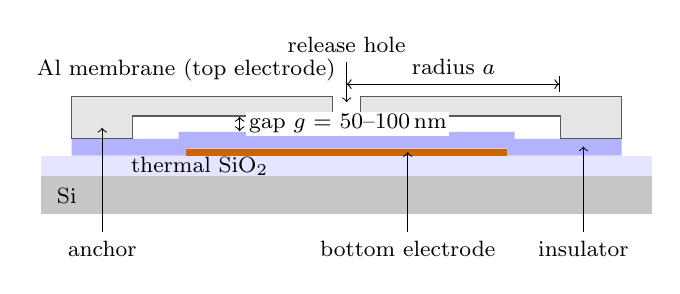
\begin{tikzpicture}[x=0.97cm,y=0.88cm,font=\footnotesize]
      % substrate and thermal oxide
      \fill[gray!45] (0,0) rectangle (8,0.55);
      \fill[blue!10] (0,0.55) rectangle (8,0.85);
      \node[anchor=west] at (0.08,0.27) {Si};
      \node[anchor=west] at (1.05,0.70) {thermal SiO$_2$};
      % bottom electrode, then the insulator over it
      \fill[orange!80!black] (1.9,0.85) rectangle (6.1,0.95);
      \fill[blue!30] (0.4,0.85) -- (1.9,0.85) -- (1.9,0.95) -- (6.1,0.95) -- (6.1,0.85) -- (7.6,0.85)
      -- (7.6,1.09) -- (6.2,1.09) -- (6.2,1.19) -- (1.8,1.19) -- (1.8,1.09) -- (0.4,1.09) -- cycle;
      % Al membrane with anchors and centre release hole
      \fill[gray!20,draw=gray!70!black,line width=0.4pt]
      (0.4,1.09) -- (1.2,1.09) -- (1.2,1.42) -- (3.82,1.42) -- (3.82,1.70) -- (0.4,1.70) -- cycle;
      \fill[gray!20,draw=gray!70!black,line width=0.4pt]
      (7.6,1.09) -- (6.8,1.09) -- (6.8,1.42) -- (4.18,1.42) -- (4.18,1.70) -- (7.6,1.70) -- cycle;
      % gap marker
      \draw[<->,line width=0.4pt] (2.6,1.20) -- (2.6,1.41);
      \node[anchor=west,fill=white,inner sep=1pt] at (2.68,1.305) {gap $g$ = 50--100\,nm};
      % labels
      \node[anchor=south] at (1.9,1.78) {Al membrane (top electrode)};
      \draw[->,line width=0.35pt] (4.0,2.2) node[above]{release hole} -- (4.0,1.62);
      \draw[<->|,line width=0.4pt] (4.0,1.88) -- (6.8,1.88);
      \node[above] at (5.4,1.88) {radius $a$};
      \draw[->,line width=0.35pt] (0.8,-0.25) node[below]{anchor} -- (0.8,1.25);
      \draw[->,line width=0.35pt] (4.8,-0.25) node[below]{bottom electrode} -- (4.8,0.90);
      \draw[->,line width=0.35pt] (7.1,-0.25) node[below]{insulator} -- (7.1,0.98);
    \end{tikzpicture}
  \end{minipage}\hfill
  \begin{minipage}[c]{0.355\textwidth}
    \caption{One CMUT cell in cross-section (not to scale). The gap is set by a thin photoresist layer that is dissolved through the release hole. A voltage between the membrane and the bottom electrode pulls the membrane toward the substrate.}
    \label{fig:cell}
  \end{minipage}
  \vspace{-5pt}
\end{figure}

The key design choice in our proposal is the gap: a smaller gap lowers the voltage required to drive the membrane. Still, it increases its susceptibility to sticking to the substrate during fabrication~\cite{brenner2019,gerardo2018}. A commercial ultrasound-on-a-chip uses a ${\sim}\SI{200}{nm}$ gap~\cite{rothberg2021}. We will build CMUTs with 50, 75, and \SI{100}{nm} gaps and measure how this trade-off plays out below \SI{100}{nm}. Based on plate models and preliminary reports, we expect that reducing the gap will significantly decrease the pull-in voltage, making low-voltage operation feasible. However, we also anticipate a sharp increase in stiction as the gap narrows, particularly below \SI{75}{nm}, which may limit the maximum usable membrane size. We hypothesize that optimal low-voltage performance will be balanced against a higher risk of stiction at the smallest gaps, revealing new regimes not accessible in previous work.

% =====================================================================
\section{Objectives}

\begin{enumerate}[label=\textbf{O\arabic*}, leftmargin=2.2em]
  \item \textbf{Fabricate} CMUT cells and small (8-element) arrays with 50, 75, and \SI{100}{nm} gaps.
  \item \textbf{Pull-in voltage.} Measure how the voltage at which the membrane snaps down depends on gap and membrane size, and compare with a simple plate model, $\VPI \propto g^{3/2}/a^{2}$.
  \item \textbf{Stiction.} Find the largest membrane that survives release at each gap (predicted to grow as $\sqrt{g}$).
  \item \textbf{Arrays.} Measure array uniformity and estimate its effect on steering an ultrasound beam.
\end{enumerate}

% =====================================================================
\section{Approach}

Every die has the same test structures, so each fabrication run is also a measurement. Table~\ref{tab:process} lists the steps each one uses.
\begin{itemize}
  \item \textbf{Membranes of several radii.} The largest that survives release measures the stiction limit.
  \item \textbf{Insulator-free cells.} Touch-down shorts the cell, so pull-in and stiction show up electrically.
  \item \textbf{Test chips} processed alongside calibrate the thin resist films and test the insulator.
  \item \textbf{Control}: a ${\sim}\SI{1}{\micro\meter}$-gap version built with the same process.
\end{itemize}

% =====================================================================
\section{Characterization}

Table~\ref{tab:char} provides an overview of each measurement, its tool, and objective. We intend to perform all tests in air and characterize the devices electrically, without rigorously measuring acoustic output unless time permits.

% ---- Tables 1 and 2, side by side ------------------------------------
\par\vspace{3pt}
\noindent
\begin{minipage}[t]{0.465\textwidth}
  \centering
  \captionof{table}{Fabrication sequence.}\label{tab:process}
  \footnotesize\setlength{\tabcolsep}{4pt}
  \begin{tabularx}{\linewidth}{@{}r P{1.85cm} L@{}}
    \toprule
    & \textbf{Step} & \textbf{Process} \\
    \midrule
    1 & Bottom electrodes & Pattern, evaporate Cr/Au, lift off \\
    2 & Insulator         & Pattern, deposit \SI{50}{nm} SiO$_2$, lift off \\
    3 & Gap layer         & Spin 50/75/\SI{100}{nm} diluted resist; open anchor rings \\
    4 & Membrane          & Evaporate \SI{1}{\micro\meter} Al; pattern release holes and pads \\
    5 & Release           & Dissolve resist in acetone; rinse in IPA; dry \\
    6 & Test              & 3D-print a chip holder; test; second run if time permits \\
    \bottomrule
  \end{tabularx}
\end{minipage}\hfill
\begin{minipage}[t]{0.515\textwidth}
  \centering
  \captionof{table}{What we measure and how.}\label{tab:char}
  \footnotesize\setlength{\tabcolsep}{4pt}
  \begin{tabularx}{\linewidth}{@{}L P{3.3cm} P{0.8cm}@{}}
    \toprule
    \textbf{Measurement} & \textbf{Tool} & \textbf{Obj.} \\
    \midrule
    Gap and film thickness                        & Thin-film reflectance; SEM of cross-sections & O1 \\
    Release progress                              & Optical microscope                           & O1, O3 \\
    Pull-in voltage; stuck membranes              & I--V setup                                   & O2, O3 \\
    Array capacitance and element yield           & I--V setup\newline(capacitance--voltage sweeps) & O4 \\
    Insulator breakdown (test capacitors, first)  & I--V setup                                   & --- \\
    \bottomrule
  \end{tabularx}
\end{minipage}

% =====================================================================
\section{Materials and Tools}

\begin{minipage}[t]{0.48\textwidth}
  \textbf{Materials}
  \begin{itemize}
    \item Oxidized silicon pieces
    \item Cr, Au, Al, and SiO$_2$ deposition sources
    \item AZ3312 photoresist, thinner, developer
    \item Al etchant, acetone, IPA, 3D-printing resin
  \end{itemize}
\end{minipage}\hfill
\begin{minipage}[t]{0.48\textwidth}
  \textbf{Tools}
  \begin{itemize}
    \item MLA, evaporator, sputterer
    \item Spin coater, wet bench, 3D printer
    \item Optical microscope, SEM
    \item Optical characterization setup, I--V setup
  \end{itemize}
\end{minipage}

% =====================================================================
\begingroup
\footnotesize
\renewcommand{\section}[2]{\vspace{4.5pt}\noindent{\normalsize\bfseries\scshape References}\par\vspace{0.5pt}}
\begin{multicols}{2}
\begin{thebibliography}{9}\setlength{\itemsep}{0.5pt}
  \bibitem{griggs2024} W.~S.~Griggs \emph{et~al.}, \emph{Nat.\ Neurosci.} \textbf{27}, 196 (2024).
  \bibitem{legon2014} W.~Legon \emph{et~al.}, \emph{Nat.\ Neurosci.} \textbf{17}, 322 (2014).
  \bibitem{brenner2019} K.~Brenner \emph{et~al.}, \emph{Micromachines} \textbf{10}, 152 (2019).
  \bibitem{gerardo2018} C.~D.~Gerardo, E.~Cretu, R.~Rohling, \emph{Microsyst.\ Nanoeng.} \textbf{4}, 19 (2018).
  \bibitem{rothberg2021} J.~M.~Rothberg \emph{et~al.}, \emph{Proc.\ Natl.\ Acad.\ Sci.} \textbf{118}, e2019339118 (2021).
\end{thebibliography}
\end{multicols}
\endgroup

\end{document}
